\section{Multi-task RL}\label{sec:multitask}

\subsection{Многозадачность}

Понятно, что в одной и той же среде мы можем решать много разных задач. Для одной и той же среды каждая задача --- в рамках нашего формализма MDP --- может быть задана при помощи своей функции награды.

\begin{definition}
Для данной среды $(\St, \A, \Trans)$ \emph{набором подзадач} будем называть множество $\G$, элементы $g \in \G$ которого имеют уникальное признаковое описание, для которых задана функция награды $r^g(s, a)$ (и, возможно, свой набор терминальных состояний $\St^+_g$).
\end{definition}

Пусть наша цель --- научиться в среде решать не одну задачу, а много. Сформулируем задачу так. Нам дан набор подзадач и некоторое распределение над задачами $p(g)$. Будем считать, что в начале эпизода нам сэмплируется случайная задача, и дальше в этом эпизоде мы должны решать её. Оптимизировать будем среднюю награду <<по задачам>>:
\begin{equation}\label{multitask}
\E_{g \sim p(g)} \E_{\Traj \sim \pi} \sum_{t \ge 0}\gamma^t r^g_t \to \max_{\pi}
\end{equation}

\begin{example}
Типичный пример $g$ --- координаты целевой точки, до которой нужно добраться, или в которую нужно что-то переместить.
\end{example}

\begin{example}
Например, если вы учите робота ходить, то вы можете в качестве $g$ брать направления движения. Тогда функция награды будет поощрять робота за, например, перемещение по вектору $g$, а сам этот вектор будет генерироваться случайно в начале эпизода.
\end{example}

\begin{theorem}
Задачу \eqref{multitask} можно свести к обычному MDP, добавив в состояния информацию о текущей решаемой задаче.
\begin{proof}
Действительно, пусть $\hat{\St} \coloneqq \St \times \G$. Пусть начальное состояние будет определяться стохастично как $(s_0, g)$, где $s_0$ --- начальное состояние нашей исходной среды (без ограничения общности считаем его фиксированным), $g \sim p(g)$. В функцию переходов $\hat{\Trans}$ просто добавим информацию о текущей решаемой задачи:
\begin{equation}\label{transition_indep_from_goal}
p(s' \mid s, g, a) \coloneqq p(s' \mid s, a), \quad g' \HM\coloneqq g
\end{equation} 
Функцию награды определим как $\hat{r}(s, g, a) \coloneqq r^g(s, a)$. Наконец, терминальными определим все пары $\{ (s, g) \mid g \in \St^+_g\}$. Тогда оптимизируемый функционал для MDP $(\hat{\St}, \A, \hat{\Trans}, \hat{r})$ в точности совпадает с \eqref{multitask}.
\end{proof}
\end{theorem}

Итак, придуманная постановка задачи просто переводит нас в другое MDP: формально <<ничего не изменилось>>. Но мы поняли важную вещь: решение многих задач в среде <<параллельно>> эквивалентно хранению в состояниях информации о текущей решаемой задачи. Коли так, и если у задач есть признаковое описание (это было важное предположение), то мы можем искать оценочные функции всего набора совместно: например, моделировать $Q^*(s, g, a)$, где описание $g$ решаемой задачи поступает модели на вход вместе с $s$. Это в точности эквивалентно тому, что $g$ хранилось бы как часть описание состояний; тогда оно тоже бы поступало на вход оценочным функциям.

\begin{definition}
Модель для аппроксимации оценочной функций сразу для набора подзадач называется \emph{универсальной оценочной функцией} (universal value function). Аналогично можно рассматривать <<\emph{универсальную стратегию}>> $\pi(a \mid s, g)$.
\end{definition}

\subsection{Мета-контроллеры}

Обсудим, как можно формализм мультизадачности применить в обычной задаче RL. Часто в алгоритме у нас встречаются важные гиперпараметры, которые трудно заранее подобрать. Выделим два примера: коэффициент дисконтирования $\gamma$ и коэффициент масштабирования внутренней мотивации $\alpha$ из уравнения \eqref{sumgoal}. Вместо того, чтобы подбирать эти параметры <<по сеточке>>, мы можем запустить multi-task RL, где $g$ --- пара $\gamma, \alpha$. Далее, вместо оценочных функций, например, $Q^*(s, a)$, будем учить универсальные оценочные функции $Q^*(s, a, \gamma, \alpha)$. Такая функция будет выдавать для данной пары $s, a$ будущую награду с учётом поданного на вход дисконтирования $\gamma$ и масштаба бонуса внутренней мотивации $\alpha$. Такое обобщение хорошо и само по себе, поскольку снабдит модель оценочной функции вспомогательными градиентами.

Мета-контроллеры могут помочь автоматически определить, для каких именно значений гиперпараметров $\gamma, \alpha$ алгоритму легче всего максимизировать среднюю внешнюю награду за эпизод. Для этого перед каждым очередным запуском эпизода обучения многорукий бандит (раздел \ref{sec:bandistssection}) выбирает $\gamma, \alpha$, которые будут использоваться в текущем эпизоде обучения для сбора данных. После окончания каждого эпизода бандит считает наградой, полученной <<из данного автомата>> суммарную (не дисконтированную) внешнюю награду, то есть истинное значение счёта игры.

Этот трюк может успешно применяться для автоматического подбора гиперпараметров прямо по ходу самого обучения. Можно смотреть на это так: будто в формуле \eqref{multitask} мы начинаем учить <<хорошее>> $p(g)$.

\subsection{Переразметка траекторий}\label{subsec:hindsight}

Рассмотрим обучение универсальной оптимальной Q-функции для набора подзадач $\G$. Для данной тройки $s, g, a$ при имеющемся сэмпле следующего состояния $s'$ мы можем обучаться на стандартный одношаговый таргет:
$$y(s, g, a) \coloneqq r^g(s, a) + \gamma \max_{a'} Q^*(s', g, a')$$

Сделаем важное наблюдение: допустим, нам известна функция награды $r$. Это довольно типичная ситуация в тех случаях, когда каким-то образом задан целый набор подзадач в среде, но при необходимости её также можно учить по собираемым сэмплам. Тогда заметим, что мы можем для имеющегося сэмпла $s' \sim p(s' \mid s, a)$ посчитать значение целевой переменной $y(s, \hat{g}, a)$ для любых $\hat{g} \in \G$. Действительно: в силу \eqref{transition_indep_from_goal} вне зависимости от того, какую цель преследовал агент, собравший переход $(s, g, a, r, s', \done)$, информацию о следующем состоянии $s'$ --- сэмпл из функции переходов --- можно использовать для обучения оценочной функции для любой задачи:
$$y(s, \hat{g}, a) \coloneqq r^{\hat{g}}(s, a) + \gamma \max_{a'} Q^*(s', \hat{g}, a')$$

\begin{example}
Допустим, вы стояли перед дверью ($s$), хотели пиццу ($g$), открыли дверь ($a$) и дверь открылась ($s'$). Тогда если бы вы, стоя перед дверью ($s$) хотели бы мороженное ($\hat{g}$) и открыли дверь ($a$), дверь всё равно бы открылась ($s'$ не изменился).
\end{example}

Это открывает путь к \emph{трансферу знаний} (transfer learning): опыт, собранный при решении одной задачи, можно использовать для обучения решению других задач. Понятно, что мы так можем <<переразметить>> не только переход, но целую траекторию.

\begin{definition}
Замена в собранной траектории цели $g$ на другую цель $\hat{g}$ и наград $r^g(s, a)$ на $r^{\hat{g}}(s, a)$ называется \emph{переразметкой траектории} (trajectory relabeling). 
\end{definition}

В простейшем случае, если размерность пространства задач $\G$ не очень большое, можно <<сохранить>> в буфере (или использовать для on-policy обучения в зависимости от использующегося алгоритма) переразмеченные траектории для всех $\hat{g}$. Однако, если $\G$ континуально, или поднабор задач богатый, то необходимо выбирать, для каких $\hat{g}$ проводить переразметку. Например, можно посэмплировать $\hat{g}$ случайно; можно ли придумать что-то умнее?

\subsection{Hindsight Experience Replay (HER)}

\needspace{5\baselineskip}
\begin{wrapfigure}{l}{0.3\textwidth}
\vspace{-0.7cm}
\centering
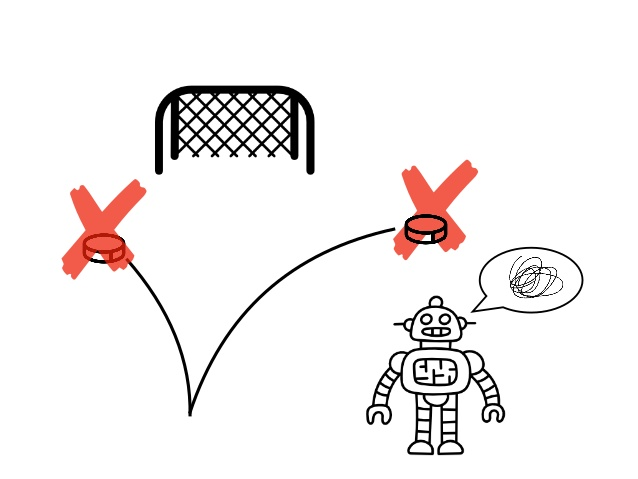
\includegraphics[width=0.3\textwidth]{Images/HERres/HERres4.jpg}
\vspace{-0.7cm}
\end{wrapfigure}

Идею hindisght-переразметки сначала обсудим на примере частного случая задачи RL, задачи поиска \eqref{searchreward}. Мы уже обсуждали как можно справляться с этой задачей при помощи внутренней мотивации (раздел \ref{subsec:intrinsic_motivation}); сейчас мы сможем при помощи формализма мультизадачности придумать ещё один интересный способ.

Пусть мы предприняли попытку достичь цели и, через некоторое число шагов, остановились в состоянии $\bar{s}$, так и не справившись с задачей. Очередной отрицательный пример с константной наградой не позволяет нам начать ничему обучаться... хотя постойте-ка. Мы же достигли состояния $\bar{s}$! Давайте положим в него виртуальный тортик. За виртуальный тортик выдадим себе виртуальную +1. Теперь у нас есть положительный пример: если бы мы хотели достичь состояния $\bar{s}$, достичь виртуального тортика, то в ходе этой последней попытки мы всё делали правильно. Другими словами, мы говорим: я так и задумывал изначально, я с самого начала хотел добраться до тортика. В английском языке подобному <<мышлению задним числом>> соответствует выражение <<\emph{in hindsight}>>, и это слово часто используется для названия алгоритмов с этой идеей. 

\needspace{5\baselineskip}
\begin{wrapfigure}[6]{r}{0.35\textwidth}
\vspace{-0.5cm}
\begin{adjustwidth}{-0.4cm}{}
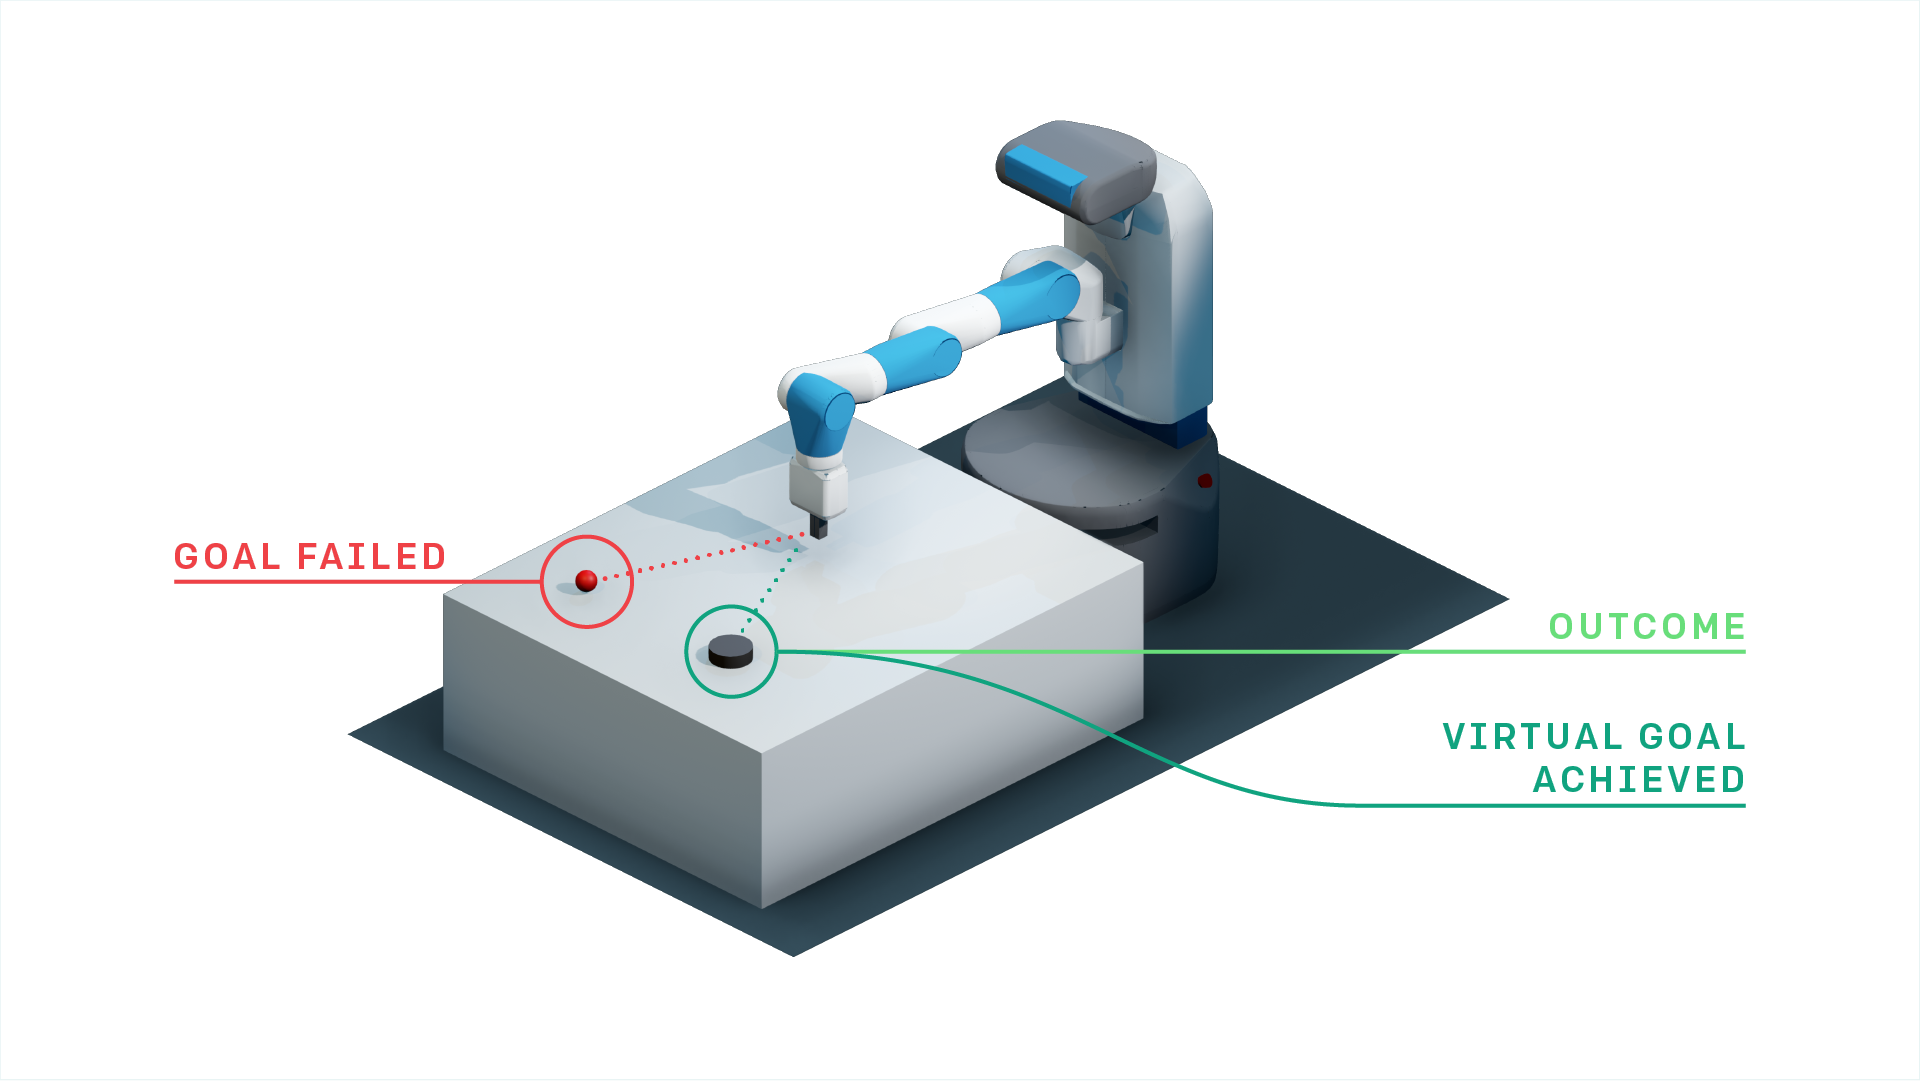
\includegraphics[width=0.4\textwidth]{Images/virtualgoal.png}
\end{adjustwidth}
%\vspace{-1.5cm}
\end{wrapfigure}

\emph{Hindsight Experience Replay} может быть формализован следующим образом. Формально мы зададимся набором подзадач, и все подзадачи будут являться задачи поиска \eqref{searchreward}. Тогда каждая функция награды $r^g$ однозначно задаётся множеством терминальных состояний --- подмножеством $\St^+_g \subseteq \St$. 

\begin{definition}
Задачей \emph{навигации} (navigation) в среде с пространством состояний $\St$ будем называть набор подзадач $\G \equiv \St$, в котором для решения задачи $g \in \St$ необходимо достичь состояния из $\St^+_g$ --- близких по некоторой метрике состояний к $g$.
\end{definition}

\begin{example}
Самый простой и доступный всегда вариант --- взять вырожденную метрику, и таким образом рассматривать $\St^+_g \coloneqq \{g\}$. В детерминированных средах такая задача даже осмысленна, но дальнейший алгоритм сработает с такой метрикой и для стохастичных сред (поскольку in hindisight мы всегда берём реально достигнутые состояния). Но во многих задачах естественным образом возникают и другие метрики. Например, если вы перемещаете шайбу, и цель задаётся координатами, то можно в качестве метрики взять расстояние от шайбы до цели. 
\end{example}

Навигация --- это в некотором смысле <<полный>> набор подзадач: для любого состояния $s$ найдётся задача, для которой оно является терминальным (победным): $\exists \St^+_g \in \G \colon s \in \St^+_g$. Это важно для нас, чтобы мы для любой траектории могли найти задачу $g \HM\in \G$, <<решением>> которой эта траектория является.

Допустим, обучается какой-либо off-policy алгоритм, работающий с реплей буфером. Все модели в алгоритме, принимающие на вход $s$, теперь также будут принимать описание задачи $g$. Будем сэмплировать $g \sim p(g)$, как и раньше, в начале эпизода; или же, если этот вариант нам недоступен, пытаться решить исходную задачу с <<истинной>> целью, которую обозначим за $g^*$. 

\begin{remark}
Допустим, нам поставили весьма конкретную задачу научиться достигать $\St^+ \subseteq \St$. Возможно, мы не знаем даже описания целевых терминальных состояний (<<выйти из лабиринта>>, а где выход --- непонятно); тогда положим описание этой <<истинной>> задачи каким-нибудь специальным вектором $g^*$.
\end{remark}

\needspace{15\baselineskip}
\begin{wrapfigure}{r}{0.35\textwidth}
\vspace{-0.4cm}
\centering
\animategraphics[controls, width=\linewidth]{1}{Images/HER/HER-}{1}{5}
\vspace{-0.5cm}
\end{wrapfigure}

Допустим, на очередном шаге мы не смогли решить задачу $g^*$, и очередной эпизод закончился в состоянии $\bar{s}$. Собранные переходы с $r = 0$ и $\done = 0$ отправились в буфер. Но мы понимаем, что если бы мы хотели бы решить задачу $g \colon \bar{s} \in \St^+_g$, то данная траектория была победной. Тогда на последнем шаге, в конце эпизода, мы получили бы награду +1 и индикатор завершения эпизода $\done = 1$. Итак, мы можем переразметить траекторию новой целью $g$, и добавить переразмеченную траекторию в буфер.

В итоге, если раньше в буфер попадали только примеры с нулевым (константным) сигналом, и обучение было невозможно, теперь же у нас есть примеры с информативным сигналом.  

Здесь важно озаботиться богатством реплей буфера для решения вспомогательных задач. Нужно иметь примеры не только правильных последних шагов, но и всех остальных; важно также не перебить вспомогательными задачами буфер и оставить примеры с целью $g^*$, чтобы алгоритм в конечном счёте научился решать и её.

\begin{exampleBox}[righthand ratio=0.3, sidebyside, sidebyside align=center, lower separated=false]{}
Допустим, вы хотите научиться бить по шайбе так, чтобы она попадала в ворота. Вы бьёте по шайбе, но не попадаете; информативного сигнала нет. Тем не менее, люди каким-то образом способны учиться на подобных ошибках, не имея успешных примеров. Вероятно, мы в реальности мыслим в терминах <<левее-правее>>, которых в формализме MDP нет. С точки зрения HER, мы просто учимся попадать в ту же точку, в которую действительно попали, поскольку у нас есть пример того, как это делается; <<если бы ворота были в этой точке, я бы попал>>. И так, обучаясь попадать в различные точки, модель может обобщится на разные $g$, и однажды попадёт в том числе в реальные ворота $g^*$.

\tcblower
\animategraphics[controls, width=\linewidth]{1}{Images/HERres/HERres}{5}{9}
\end{exampleBox}

\subsection{Hindsight Relabeling}

Обобщим идею HER на произвольные multi-task задачи. Понятно, что примеры <<хорошего>> решения задачи нам намного ценнее примеров неудач: переразметкой мы боремся с тем, что в классическом машинном обучении назвали бы <<несбалансированностью выборки>>, увеличивая число примеров <<более редкого класса>>.

Итак, дан произвольный набор подзадач $r(s, a, g)$. Мы преследовали какую-то цель (неважно какую) и породили траекторию $\Traj$. Обозначим $R^g(\Traj)$ суммарную награду за траекторию с точки зрения задачи $g$. Вопрос: для каких $g \in \G$ имеет смысл переразметить эту траекторию? 

\begin{exampleBox}[label=ex:multitask]{}
Допустим, мы собирали орешки и породили такую траекторию:

\begin{center}
    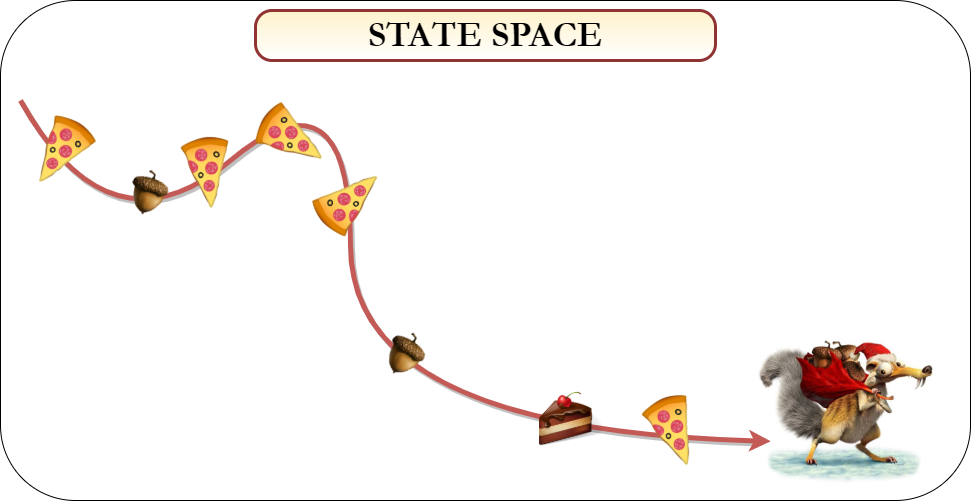
\includegraphics[width=0.7\textwidth]{Images/MultiTask1}
\end{center}

Для какой задачи данная траектория является <<информативной>>, то есть примером хорошего решения? Очевидный ответ <<для пицц>> внезапно неверен: да, мы собрали пицц больше чем орешков, но вдруг собрать 5 пицц --- это очень мало, и такая траектория наоборот является плохой с точки зрения задачи сбора пицц?

А ещё данная траектория является успешным примером задачи <<избежать львов>>, поскольку ни одного льва в траектории не было. То есть важно не сколько награды $R^g(\Traj)$ мы собрали, а сравнение этого значения с тем, сколько может набрать хорошая стратегия решения задачи $g$.
\end{exampleBox}

Переформулируем вопрос: для какой задачи $g$ из нашего параметрического семейства $r(s, a, g)$ наша траектория является экспертной? Итак, ключевое наблюдение: поиск хороших $g$ для переразметки --- это задача обратного обучения с подкреплением, которую мы обсуждали в разделе \ref{subsec_irl}. В идеях Maximum Entropy Inverse RL и лежит ответ на наш вопрос.

С точки зрения Maximum Entropy подхода (формулы \eqref{meirl}), траектория $\Traj$ является экспертной для задачи $g$ с вероятностью
$$p(\Traj \mid g) \coloneqq \frac{e^{R^g(\Traj)} \prod_{t \ge 0}p(s_{t+1} \mid s_t, a_t)}{Z(g)}$$
Заметим, что нормировочная константа для каждого $g$ своя. Рассмотрим в качестве прайора $p(g)$, из которого нам, например, приходят задачи в начале эпизодов или возьмём какое-нибудь равномерное распределение. Тогда по формуле Байеса:
\begin{equation}\label{bayes_relabeling}
p(g \mid \Traj) \propto p(\Traj \mid g)p(g) = \frac{p(g) e^{R^g(\Traj)}}{Z(g)}
\end{equation}
Часть с вероятностями переходов сократились с нормировочной константой, поскольку они общие для всех $g$. Эта формула и говорит нам, что нужно использовать для поиска хорошей переразметки $g$ не просто задачи, для которых мы собрали большую суммарную награду $R^g(\Traj)$, а отнормированную на соответствующий интеграл $Z(g)$. Именно с вероятностями \eqref{bayes_relabeling} цель $g$ можно считать <<экспертной>>.

Формула \eqref{bayes_relabeling} даёт теоретический ответ на наш вопрос, но как использовать её на практике, то есть как сэмплировать из такого распределения? Здесь придётся ограничиться эвристиками. Если $\G$ конечно и мало, то мы можем подсчитать для каждого $g$ все суммарные награды $R^g(\Traj)$, но с нормировочной константой дела обстоят плохо: 
$$Z(g) = \int\limits_{\Traj} e^{R^g(\Traj)} \prod_{t \ge 0}p(s_{t+1} \mid s_t, a_t) \diff \Traj,$$
где траектории, вообще говоря, должны быть порождены оптимальной стратегией, решающей задачу $g$; мы можем считать, что текущая универсальная стратегия $\pi(a \mid s, g)$ и является экспертной для искомого $g$. Эвристики сводятся к тому, чтобы взять какие-нибудь траектории из буфера $\Traj_1, \Traj_2 \dots \Traj_M$ и посчитать примерно среднюю награду, которую мы набираем как-нибудь так:
$$Z(g) \approx \frac{1}{M} \sum_{i = 1}^M e^{R^g(\Traj_i)}$$
Если $\G$ велико или, например, континуально, то просто для поиска хороших $g$ сэмплируется случайно несколько целей-кандидатов, и поиск хороших целей для переразметки проводится среди них.

\begin{example}
Продолжим пример \ref{ex:multitask} и посмотрим на несколько других встречавшихся траекторий из буфера.
\begin{center}
    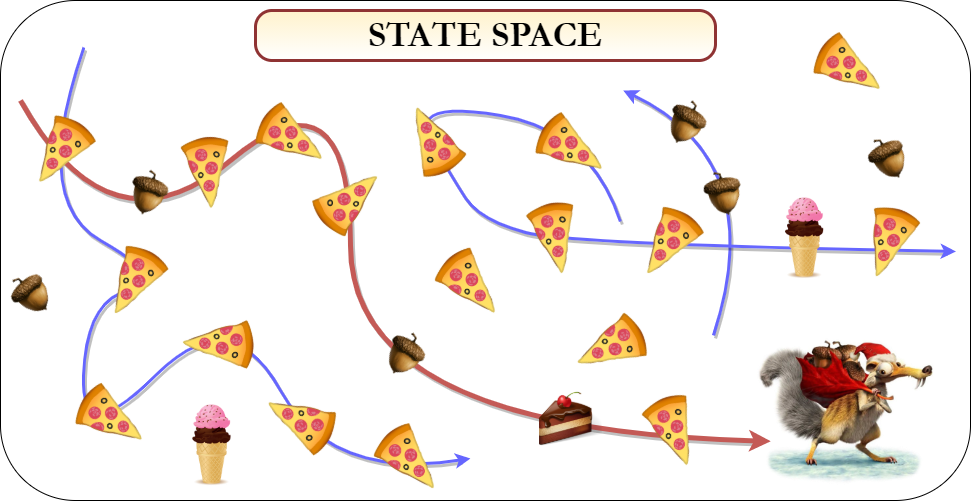
\includegraphics[width=0.7\textwidth]{Images/MultiTask3}
\end{center}
Теперь мы видим, что собрать 5 пицц --- не такое редкое явление; наша собственная стратегия когда-то уже получала даже больше. А вот до тортиков мы в засэмплированных траекториях никогда не добирались, и поэтому нашу траекторию имеет смысл переразметить для задачи <<добраться до тортика>>. Таким образом у нас в буфере появится пример сбора целого 1 тортика, что, согласно примерам других траекторий, <<много>> для этой задачи.
\end{example}